\documentclass{article}
\usepackage[utf8]{inputenc}
\usepackage{polski}
\usepackage{graphicx}


\begin{document}

\begin{titlepage}
\newcommand{\HRule}{\rule{\linewidth}{0.5mm}}
\begin{center}
\textsc{\LARGE Politechnika Warszawska}\\[0.5cm]
\textsc{\Large Wydział Matematyki i Nauk Informacyjnych}\\[1cm]

\includegraphics[width=2cm, height=2cm]{logo}\\[1cm]
\textsc{\Huge Sieci neuronowe}\\[0.5cm]
\HRule \\[0.4cm]
{ \LARGE \bfseries Rozpoznawanie i klasyfikacja pisanych cyfr przy użyciu modeli matematycznych}\\[4cm]
\begin{flushright}
\Large \emph{Autorzy:}\\[0.5cm]
Anna \textsc{Zawadzka}\\
Piotr \textsc{Waszkiewicz}\\[2.5cm]
\end{flushright} 
\vfill
{\large \today}\\[1cm]	
\end{center}
\end{titlepage}

\newpage
%----------------------------------------------------------------------------------------
\section{Opis problemu badawczego}
Problem badawczy przedstawiony na stronie \textit{https://www.kaggle.com/c/digit-recognizer} polega na rozpoznawaniu i klasyfikacji ręcznie pisanych cyfr poprzez przetwarzanie i analizę obrazów przedstawiających odpowiednie symbole. Zbiory danych zostaną zaczerpnięte z publicznej bazy danych  MNIST\cite{mnist_database}. 
\begin{center}
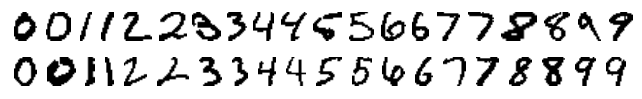
\includegraphics[width=0.49\textwidth]{native}
\end{center}

\section{Planowane do wykorzystania techniki}
Projekt zakłada realizację zadania poprzez zbadanie różnych metod, ze szczególnym uwzględnieniem różnych modeli sieci neuronowych. Na chwilę obecną planowana jest konstrukcja sieci klasyfikującej typu \textit{feed-forward} zgodnie z opisem na stronie biblioteki PyBrain\cite{pybrain}. Wykorzystane zostaną również jedne z najpopularniejszych obecnie klasyfikatorów: maszyny wektorów podpierających (SVM)\cite{CortesVapnik1995}, Lasy Losowe\cite{RF}, kNN\cite{Altman1992} oraz model regresji wielomianowej. \\

\section{Cel badań}

Celem badań jest porównanie jakości klasyfikacji dla różnych modeli matematycznych i wskazanie najskuteczniejszego klasyfikatora pod względem czasu uczenia, wydajności i jakości udzielanych odpowiedzi. Oprócz tego badania mają na celu rozszerzenie istniejącego wektora cech o nowe, unikalne wartości które polepszą jakość klasyfikacji. Przykładem takich cech może być liczba przecięć w napisanym symbolu, liczba zakończeń lub procent powierzchni zajmowanej przez narysowany symbol. W trakcie obliczeń podjęta zostanie próba odrzucenia tych cech które przeszkadzają lub pogarszają działanie modeli. Przeprowadzone badania obejmą również wybór optymalnych parametrów dla poszczególnych klasyfikatorów metodą GridSearch\cite{gridsearch}. \\


\section{Opis danych}

Zbiory danych treningowych oraz testowych pochodzą z publicznej bazy danych MNIST\cite{mnist_database}. Każdy element ze zbioru treningowego jest opisany 785 wartościami. Pierwsza liczba określa zakodowaną cyfrę (wartość z przedziału [0, 9]), kolejne 784 wartości są z przedziału [0, 255] i opisują kolory pikseli zeskanowanej cyfry w skali szarości dla obrazka o wymiarach 28x28 pikseli. Zbiór testowy w przeciwieństwie do treningowego nie zawiera informacji o reprezentowanej klasie. Zbiór treningowy i testowy zawierają odpowiednio 60,000 i 10,000 elementów. \\


\section{Sposób weryfikacji rezultatów}

Podczas ewaluacji otrzymywanych rozwiązań minimalizowana będzie funkcja błędu opisana wzorem \[ f(M, d) = e(M, d) + t(M, d) \] gdzie \textit{M} oznacza model, \textit{d} zbiór testowy, \textit{e()} współczynnik \textit{Error rate}, czyli miarę określającą stosunek źle zaklasyfikowanych elementów do wszystkich obiektów w zbiorze, oraz \textit{t()} funkcję czasu liczoną jako liczbę sekund potrzebną na realizację obliczeń.

\newpage
\begin{thebibliography}{9}
	\bibitem{mnist_database} LeCun, Y., Cortes, C., and Burges, C., \emph{The MNIST database of handwritten digits}, in: http://yann.lecun.com/exdb/mnist.
	\bibitem{RF} Breiman, L., \emph{Random Forests}. Machine Learning 45 (1), 2001
	\bibitem{CortesVapnik1995} Cortes, C., Vapnik, V., \emph{Support-vector networks}. Machine Learning 20 (3), 1995.	
	\bibitem{Altman1992} Altman N. S., \emph{An introduction to kernel and nearest-neighbor nonparametric regression}. The American Statistician 46 (3), 1992.
    \bibitem{ScholkopfWilliamsonSmola1992} Scholkopf, B., Williamson, R., Smola, A., Shawe-Taylort, J., Platt, J., \emph{Support Vector Method for Novelty Detection}, Advances in Neural Information Processing Systems 12, 1992. 
    \bibitem{WangCasasent2009} Wang, Y., Casasent, D., \emph{A Support Vector Hierarchical Method for multi-class classification and rejection}, Proc. of Int. Joint Conf. on Neural Networks, 2009.
    \bibitem{gridsearch} http://scikit-learn.org/stable/modules/grid\_search.html.
    \bibitem{pybrain} http://pybrain.org/docs/tutorial/fnn.html


\end{thebibliography}

\end{document}